\section{Definitions, notation, and preliminary lemmas}
\label{sec:definitions}

\subsection{Graph maps, densities, and sampling}
\label{subsec:graph-maps-and-sampling}

All graphs below are finite and simple.
For an integer $s\geq0$, write $[s]=\{1,\ldots,s\}$, with
$[0]=\varnothing$.
The graph $G$ denotes the ambient graph, with $n=|V(G)|\geq1$.

For graphs $J,H$, define the set of graph isomorphisms by
\begin{equation}\label{eq:graph-isomorphisms}
\operatorname{Iso}(J,H)=
\left\{\phi:V(J)\overset{\mathrm{bij}}{\longrightarrow}V(H):
(A_J)_{uv}=(A_H)_{\phi(u)\phi(v)}
\ \text{for all }u,v\in V(J)\right\}.
\end{equation}
We write $J\cong H$ if $\operatorname{Iso}(J,H)\ne\varnothing$.
For a subset $S\subseteq V(G)$, the induced subgraph is
\[
G[S]=\big(S,\{\{u,v\}\in E(G):u,v\in S\}\big).
\]

The sets of homomorphisms, injective homomorphisms, and induced embeddings
from $J$ to $G$ are, respectively,
\begin{align}
\operatorname{Hom}(J,G)
&=\left\{\phi:V(J)\longrightarrow V(G):
\{\phi(u),\phi(v)\}\in E(G)
\ \text{for every }\{u,v\}\in E(J)\right\},
\label{eq:graph-homomorphisms}\\
\operatorname{Emb}(J,G)
&=\{\phi\in\operatorname{Hom}(J,G):\phi\text{ is injective}\},
\label{eq:graph-injective-homomorphisms}\\
\operatorname{Emb}_{\mathrm{ind}}(J,G)
&=\left\{\phi:V(J)\hookrightarrow V(G):
(A_J)_{uv}=(A_G)_{\phi(u)\phi(v)}
\ \text{for all }u,v\in V(J)\right\}.
\label{eq:graph-induced-embeddings}
\end{align}
An injective homomorphism is required to preserve edges, whereas an
induced embedding preserves both edges and nonedges.

Let $s=|V(J)|$.
For $n\geq s$, write
\[
(n)_s=n(n-1)\cdots(n-s+1)=\frac{n!}{(n-s)!},
\qquad (n)_0=1.
\]
The homomorphism and injective homomorphism densities are
\begin{equation}\label{eq:graph-homomorphism-densities}
t(J,G)=\frac{|\operatorname{Hom}(J,G)|}{n^s},
\qquad
t_{\mathrm{inj}}(J,G)=\frac{|\operatorname{Emb}(J,G)|}{(n)_s}
\quad(n\geq s).
\end{equation}
To write these densities as adjacency products, label $V(J)$ by $[s]$.
Then
\begin{align}
t(J,G)
&=\frac1{n^s}
\sum_{x_1,\ldots,x_s\in V(G)}
\prod_{\{a,b\}\in E(J)}(A_G)_{x_ax_b},
\label{eq:graph-homomorphism-product}\\
t_{\mathrm{inj}}(J,G)
&=\frac1{(n)_s}
\sum_{\substack{(x_1,\ldots,x_s)\in V(G)^s\\
x_a\ne x_b\ \text{for }a\ne b}}
\prod_{\{a,b\}\in E(J)}(A_G)_{x_ax_b}.
\label{eq:graph-injective-product}
\end{align}
Each product is the indicator that the map $a\mapsto x_a$ preserves
all edges of $J$; the second sum restricts these maps to injections.
Empty products are taken to be $1$.
For $n\geq s$, the induced-subgraph density is
\begin{equation}\label{eq:graph-induced-density}
p(J,G)=
\frac{\big|\{S\subseteq V(G):|S|=s,\ G[S]\cong J\}\big|}
{\binom ns}.
\end{equation}

\paragraph{Sampling on positions.}
For an integer $h\geq0$, let $\boldsymbol{X}=(X_1,\ldots,X_h)$ have independent
uniform coordinates in $V(G)$.
Thus $\boldsymbol{X}$ is uniformly distributed on $V(G)^h$, with replacement.
Define the graph on the sampled positions by
\begin{equation}\label{eq:sampled-position-graph}
G_{\boldsymbol{X}}=\left([h],\
\left\{\{a,b\}:1\leq a<b\leq h,
\ \{X_a,X_b\}\in E(G)\right\}\right).
\end{equation}
In particular,
\begin{equation}\label{eq:sampled-adjacency}
(A_{G_{\boldsymbol{X}}})_{ab}=(A_G)_{X_aX_b}
\qquad(a,b\in[h]).
\end{equation}
Expectations and probabilities in this sampling rule are
\begin{equation}\label{eq:sampled-expectation}
\E_Xf(\boldsymbol{X})=\frac1{n^h}\sum_{\boldsymbol{X}\in V(G)^h}f(\boldsymbol{X}),
\qquad
\Pr(\boldsymbol{X}\in\mathcal A)=\frac{|\mathcal A|}{n^h}
\quad\big(\mathcal A\subseteq V(G)^h\big).
\end{equation}
For $s\in\{0,\ldots,8\}$, let $\mathcal G_s$ be the set of all
triangle-free graphs with vertex set $[s]$, that is,
\begin{equation}\label{eq:triangle-free-labeled-graphs}
\mathcal G_s=
\left\{([s],E):
\begin{array}{l}
E\subseteq\{\{a,b\}:1\leq a<b\leq s\},\\
([s],E)\text{ is triangle-free}
\end{array}\right\}.
\end{equation}
Clearly, graph isomorphism is an equivalence relation on $\mathcal G_s$.
Let $\mathcal T_s\subseteq\mathcal G_s$ be a system of representatives
for this equivalence relation; that is, for every $J\in\mathcal G_s$,
\begin{equation}\label{eq:triangle-free-representatives}
\big|\{H\in\mathcal T_s:J\cong H\}\big|=1.
\end{equation}
If $G$ is triangle-free, then $G_{\boldsymbol{X}}$ is triangle-free.
Consequently, for $0\leq h\leq8$,
\begin{equation}\label{eq:sampled-graph-partition}
V(G)^h=
\bigsqcup_{H\in\mathcal T_h}
\{\boldsymbol{X}\in V(G)^h:G_{\boldsymbol{X}}\cong H\},
\qquad
\sum_{H\in\mathcal T_h}\Pr(G_{\boldsymbol{X}}\cong H)=1.
\end{equation}

The following identity relates homomorphism densities in the ambient
graph to injective homomorphism densities in the sampled graphs.
\begin{lemma}\label{lem:sampled-density-identity}
Let $G$ be a finite simple triangle-free graph of order $n\geq1$,
let $1\leq h\leq8$, and let $J$ be a finite simple graph of order
$s\leq h$, including $s=0$.
For a random tuple $\boldsymbol{X}=(X_1,\ldots,X_h)\in V(G)^h$, where the coordinates
$X_i$ are independent and uniformly distributed on $V(G)$, we have
\begin{equation}\label{eq:sampled-density-identity}
t(J,G)=\E_Xt_{\mathrm{inj}}(J,G_{\boldsymbol{X}})
=\sum_{H\in\mathcal T_h}t_{\mathrm{inj}}(J,H)\Pr(G_{\boldsymbol{X}}\cong H).
\end{equation}
\end{lemma}
\begin{proof}
Label $V(J)$ by $[s]$ and fix an injection $\phi:[s]\hookrightarrow[h]$.
The random variables $X_{\phi(1)},\ldots,X_{\phi(s)}$ are independent
and uniform on $V(G)$, because $\phi$ selects different positions.
Using \eqref{eq:sampled-adjacency} and
\eqref{eq:graph-homomorphism-product}, we obtain
\begin{align*}
\E_{\boldsymbol{X}}\prod_{\{a,b\}\in E(J)}(A_{G_{\boldsymbol{X}}})_{\phi(a)\phi(b)}
&=\E_{\boldsymbol{X}}\prod_{\{a,b\}\in E(J)}(A_G)_{X_{\phi(a)}X_{\phi(b)}}\\
&=\frac1{n^s}\sum_{x_1,\ldots,x_s\in V(G)}
  \prod_{\{a,b\}\in E(J)}(A_G)_{x_ax_b}\\
&=t(J,G).
\end{align*}
The graph $G_{\boldsymbol{X}}$ has $h$ vertices, and there are $(h)_s$ injections
from $[s]$ to $[h]$.
By \eqref{eq:graph-injective-product} and linearity of expectation,
\begin{align*}
\E_Xt_{\mathrm{inj}}(J,G_{\boldsymbol{X}})
&=\frac1{(h)_s}\sum_{\phi:[s]\hookrightarrow[h]}
  \E_{\boldsymbol{X}}\prod_{\{a,b\}\in E(J)}(A_{G_{\boldsymbol{X}}})_{\phi(a)\phi(b)}\\
&=\frac1{(h)_s}\sum_{\phi:[s]\hookrightarrow[h]}t(J,G)
=t(J,G).
\end{align*}
This proves the first equality in \eqref{eq:sampled-density-identity}.

Since $t_{\mathrm{inj}}(J,\cdot)$ is invariant under graph isomorphism,
the partition in \eqref{eq:sampled-graph-partition} gives
\begin{align*}
\E_Xt_{\mathrm{inj}}(J,G_{\boldsymbol{X}})
&=\E_{\boldsymbol{X}}\left[\sum_{H\in\mathcal T_h}
  t_{\mathrm{inj}}(J,H)\ind_{\{G_{\boldsymbol{X}}\cong H\}}\right]\\
&=\sum_{H\in\mathcal T_h}t_{\mathrm{inj}}(J,H)
  \E_{\boldsymbol{X}}\ind_{\{G_{\boldsymbol{X}}\cong H\}}\\
&=\sum_{H\in\mathcal T_h}t_{\mathrm{inj}}(J,H)\Pr(G_{\boldsymbol{X}}\cong H).
\end{align*}
This proves the second equality.
\end{proof}

\subsection{Labeled graphs and the counting matrices}
\label{subsec:labeled-graphs-and-counts}

A type of order $k$ is a triangle-free graph
$\sigma=([k],E(\sigma))$.
A $\sigma$-labeled graph is a pair $(J,\theta)$, where $J$ is a
triangle-free graph and
\[
\theta\in\operatorname{Emb}_{\mathrm{ind}}(\sigma,J).
\]
The vertex $\theta(i)$ carries label $i$ for each $i\in[k]$.
For two $\sigma$-labeled graphs, define
\begin{equation}\label{eq:labeled-graph-isomorphism}
(J,\theta)\cong_\sigma(J',\theta')
\quad\Longleftrightarrow\quad
\{\phi\in\operatorname{Iso}(J,J'):
\phi\circ\theta=\theta'\}\ne\varnothing.
\end{equation}
Thus an isomorphism of labeled graphs preserves each specified label.
The relation $\cong_\sigma$ is an equivalence relation.

For $0\leq k\leq\ell\leq8$, let
$\iota:[k]\hookrightarrow[\ell]$ be the inclusion map $\iota(i)=i$.
Define
\begin{align}
\widehat{\mathcal G}_{\sigma,\ell}
&=\{(J,\iota):J\in\mathcal G_\ell,
  \ \iota\in\operatorname{Emb}_{\mathrm{ind}}(\sigma,J)\}\notag\\
&=\{(J,\iota):J\in\mathcal G_\ell,\ J[[k]]=\sigma\}.
\label{eq:labeled-graph-collection}
\end{align}
Here the first $k$ vertices have labels $1,\ldots,k$.
Every $\sigma$-labeled graph with $\ell$ vertices is isomorphic to an
element of \eqref{eq:labeled-graph-collection}: relabel $\theta(i)$ as
$i$ and give the remaining vertices the vertex names $k+1,\ldots,\ell$.
For the pairs in \eqref{eq:labeled-graph-collection}, the isomorphisms
in \eqref{eq:labeled-graph-isomorphism} fix $1,\ldots,k$ pointwise.

Let $\mathcal F_{\sigma,\ell}\subseteq
\widehat{\mathcal G}_{\sigma,\ell}$ be a system of representatives
for $\cong_\sigma$, and denote each representative pair by a single
symbol $P$. Thus, for every
$(J,\iota)\in\widehat{\mathcal G}_{\sigma,\ell}$,
\begin{equation}\label{eq:labeled-flag-representatives}
\big|\{P\in\mathcal F_{\sigma,\ell}:
(J,\iota)\cong_\sigma P\}\big|=1.
\end{equation}
We call the elements of $\mathcal F_{\sigma,\ell}$ the
$\sigma$-flags of order $\ell$.
Each flag has $k$ labeled vertices and $\ell-k$ unlabeled vertices.

For the counting matrices used below, take
\begin{equation}\label{eq:counting-flag-order}
\sigma\in\mathcal T_k,\qquad 0\leq k\leq6,
\qquad \ell=\left\lfloor\frac{8+k}{2}\right\rfloor.
\end{equation}
Then $2\ell-k\leq8$.
Let $H$ be a triangle-free graph with $|V(H)|=8$, and let
$P,P'\in\mathcal F_{\sigma,\ell}$.
For a map $\rho:[8]\to V(H)$ and a set $S\subseteq[8]$, write
$\rho(S)=\{\rho(i):i\in S\}$ and write $\rho|_{[k]}$ for the
restriction $i\mapsto\rho(i)$ on $[k]$.
Define
\begin{equation}\label{eq:labeled-ordering-count}
C_H^\sigma(P,P')=
\left|\left\{\rho:
\begin{array}{l}
\rho:[8]\overset{\mathrm{bij}}{\longrightarrow}V(H),\\
(A_H)_{\rho(i)\rho(j)}=(A_\sigma)_{ij}
\quad(1\leq i<j\leq k),\\
(H[\rho([\ell])],\rho|_{[k]})\cong_\sigma P,\\
(H[\rho([k]\cup\{\ell+1,\ldots,2\ell-k\})],\rho|_{[k]})
\cong_\sigma P'
\end{array}\right\}\right|.
\end{equation}
Figure~\ref{fig:flag-ordering} shows an example of a bijection $\rho$
satisfying the conditions in \eqref{eq:labeled-ordering-count}.
Fix an ordering of $\mathcal F_{\sigma,\ell}$ and use it for both the
rows and the columns of the square matrix
\[
C_H^\sigma=
\big(C_H^\sigma(P,P')\big)_{P,P'\in\mathcal F_{\sigma,\ell}}.
\]
Clearly, $C_H^\sigma(P,P')=C_H^\sigma(P',P)$ for all
$P,P'\in\mathcal F_{\sigma,\ell}$, so $C_H^\sigma$ is symmetric.

In \eqref{eq:labeled-ordering-count}, the two flags use the same
labeled positions $[k]$ and the disjoint unlabeled position sets
\[
\{k+1,\ldots,\ell\},
\qquad
\{\ell+1,\ldots,2\ell-k\}.
\]
The remaining $8-2\ell+k$ positions are unused by either flag.
The definition imposes no condition on edges between the two unlabeled
groups or on edges incident with unused positions.

\begin{figure}[htbp]
\centering
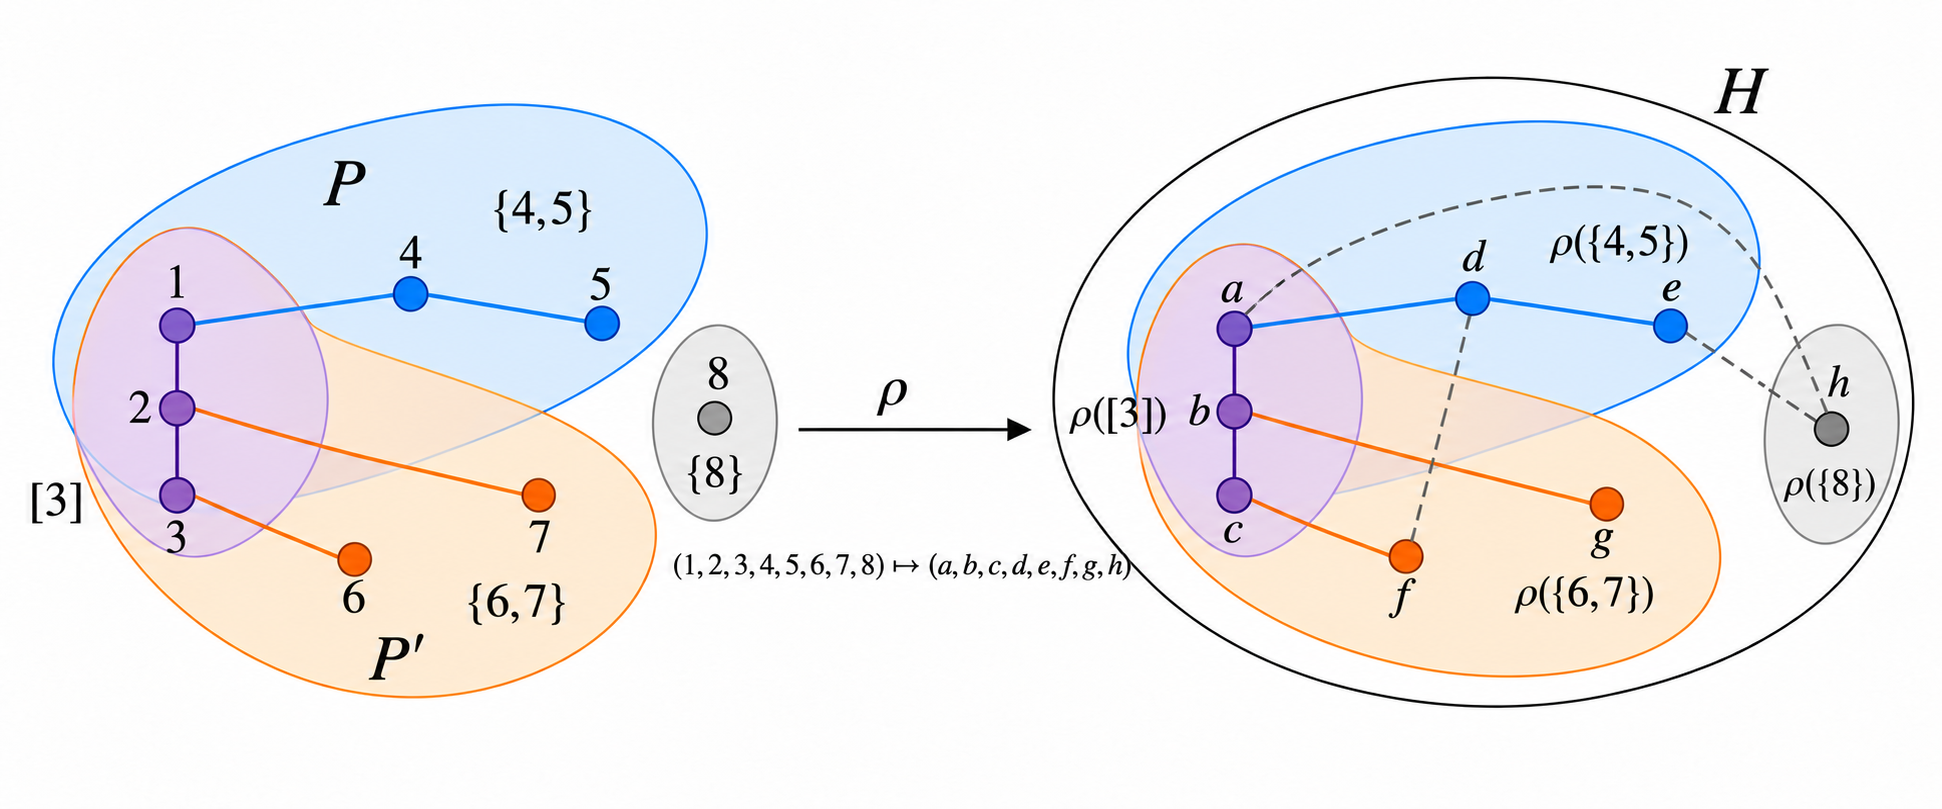
\includegraphics[width=\textwidth]{images/flag-ordering-structured-example.png}
\caption{An admissible bijection for $k=3$ and $\ell=5$.
The purple root path is $\sigma$; the blue and orange regions represent
$P$ and $P'$, respectively, and position $8$ is unused by either flag.
The gray dashed edges $ah$, $df$, and $eh$ are actual edges of $H$
unconstrained by the two flags.}
\label{fig:flag-ordering}
\end{figure}
\FloatBarrier

We now relate these counts to probabilities in the ambient graph $G$.
Fix a triangle-free graph $G$ of order $n\geq1$.
For any tuple $\boldsymbol{r}=(r_1,\ldots,r_k)\in V(G)^k$, let $G_{\boldsymbol{r}}$ be the graph
on $[k]$ given by the same rule as
\eqref{eq:sampled-position-graph}; thus
$(A_{G_{\boldsymbol{r}}})_{ij}=(A_G)_{r_ir_j}$.
For $\boldsymbol{Y}=(Y_1,\ldots,Y_{\ell-k})\in V(G)^{\ell-k}$, write
\[
(\boldsymbol{r},\boldsymbol{Y})=(r_1,\ldots,r_k,Y_1,\ldots,Y_{\ell-k}).
\]
For a flag $P\in\mathcal F_{\sigma,\ell}$, define
\begin{equation}\label{eq:conditional-probability}
\Pr(P\mid \boldsymbol{r})=
\begin{cases}
\displaystyle
\frac{\big|\{\boldsymbol{Y}\in V(G)^{\ell-k}:
(G_{(\boldsymbol{r},\boldsymbol{Y})},\iota)\cong_\sigma P\}\big|}{n^{\ell-k}},
&G_{\boldsymbol{r}}=\sigma,\\[6pt]
0,&G_{\boldsymbol{r}}\ne\sigma.
\end{cases}
\end{equation}
When $G_{\boldsymbol{r}}=\sigma$, this is the probability that
$(G_{(\boldsymbol{r},\boldsymbol{Y})},\iota)\cong_\sigma P$, where the coordinates of
$\boldsymbol{Y}=(Y_1,\ldots,Y_{\ell-k})$ are independent and uniformly distributed
on $V(G)$.
The map $\iota$ labels position $i$ by $i$ for $i\in[k]$.
For a block of length zero, $V(G)^0$ consists of the unique empty tuple.

For $P,P'\in\mathcal F_{\sigma,\ell}$, define the event
\begin{equation}\label{eq:joint-event}
\mathcal A^\sigma_{P,P'}=
\left\{\boldsymbol{x}=(x_1,\ldots,x_8)\in V(G)^8:
\begin{array}{l}
G_{(x_1,\ldots,x_k)}=\sigma,\\
(G_{(x_1,\ldots,x_\ell)},\iota)\cong_\sigma P,\\
(G_{(x_1,\ldots,x_k,x_{\ell+1},\ldots,x_{2\ell-k})},\iota)
\cong_\sigma P'
\end{array}\right\}.
\end{equation}

\begin{samepage}
\begin{lemma}\label{lem:exact-flag-square}
Let $G$ be a finite simple triangle-free graph of order $n\geq1$,
and let $\boldsymbol{X}=(X_1,\ldots,X_8)\in V(G)^8$, where the coordinates $X_i$
are independent and uniformly distributed on $V(G)$.
Fix $\sigma\in\mathcal T_k$, with $0\leq k\leq6$, let
$\ell=\lfloor(8+k)/2\rfloor$, and set $\boldsymbol{r}=(X_1,\ldots,X_k)$.
Then, for all $P,P'\in\mathcal F_{\sigma,\ell}$,
\begin{align}
\frac1{8!}\sum_{H\in\mathcal T_8}
\Pr(G_{\boldsymbol{X}}\cong H)C_H^\sigma(P,P')
&=\Pr\big(\boldsymbol{X}\in\mathcal A^\sigma_{P,P'}\big)\notag\\
&=\E_{\boldsymbol{r}}\left[\ind_{\{G_{\boldsymbol{r}}=\sigma\}}
\Pr(P\mid \boldsymbol{r})\Pr(P'\mid \boldsymbol{r})\right].
\label{eq:flag-entry-average}
\end{align}
Consequently,
\begin{equation}\label{eq:averaged-count-psd}
M_G^\sigma:=\sum_{H\in\mathcal T_8}\Pr(G_{\boldsymbol{X}}\cong H)C_H^\sigma
\quad\text{is positive semidefinite}.
\end{equation}
\end{lemma}
\end{samepage}
\begin{proof}
Let $S_8=\{\rho:[8]\overset{\mathrm{bij}}{\longrightarrow}[8]\}$.
For $\boldsymbol{X}=(X_1,\ldots,X_8)\in V(G)^8$ and $\rho\in S_8$,
write
\[
\boldsymbol{X}\circ\rho=(X_{\rho(1)},\ldots,X_{\rho(8)}).
\]
Composition with a graph isomorphism gives a bijection between the
orderings counted in \eqref{eq:labeled-ordering-count}, so
$G_{\boldsymbol{X}}\cong H$ implies
$C_{G_{\boldsymbol{X}}}^\sigma=C_H^\sigma$.
By \eqref{eq:labeled-ordering-count},
\eqref{eq:conditional-probability}, \eqref{eq:joint-event},
and \eqref{eq:sampled-graph-partition},
\begin{align*}
&\frac1{8!}\sum_{H\in\mathcal T_8}
\Pr(G_{\boldsymbol{X}}\cong H)C_H^\sigma(P,P')\\
&=\frac1{8!}\sum_{H\in\mathcal T_8}
\E_{\boldsymbol{X}}\left[
\ind_{\{G_{\boldsymbol{X}}\cong H\}}C_H^\sigma(P,P')\right]\\
&=\frac1{8!}\E_{\boldsymbol{X}}\left[
\sum_{H\in\mathcal T_8}
\ind_{\{G_{\boldsymbol{X}}\cong H\}}C_H^\sigma(P,P')\right]\\
&=\frac1{8!}\E_{\boldsymbol{X}}
C_{G_{\boldsymbol{X}}}^\sigma(P,P')\displaybreak[1]\\
&=\frac1{8!\,n^8}\sum_{\boldsymbol{X}\in V(G)^8}
\left|\left\{\rho\in S_8:
\boldsymbol{X}\circ\rho\in\mathcal A^\sigma_{P,P'}\right\}\right|\\
&=\frac1{8!\,n^8}
\left|\left\{(\boldsymbol{X},\rho)\in V(G)^8\times S_8:
\boldsymbol{X}\circ\rho\in\mathcal A^\sigma_{P,P'}\right\}\right|\\
&=\frac1{8!\,n^8}\sum_{\boldsymbol{Y}\in\mathcal A^\sigma_{P,P'}}
\left|\left\{(\boldsymbol{X},\rho)\in V(G)^8\times S_8:
\boldsymbol{X}\circ\rho=\boldsymbol{Y}\right\}\right|\\
&=\frac1{8!\,n^8}\sum_{\boldsymbol{Y}\in\mathcal A^\sigma_{P,P'}}
\sum_{\rho\in S_8}
\underbrace{\left|\left\{\boldsymbol{X}\in V(G)^8:
\boldsymbol{X}=\boldsymbol{Y}\circ\rho^{-1}\right\}\right|}_{=1}\\
&=\frac1{8!\,n^8}\sum_{\boldsymbol{Y}\in\mathcal A^\sigma_{P,P'}}
\sum_{\rho\in S_8}1\\
&=\frac1{8!\,n^8}\sum_{\boldsymbol{Y}\in\mathcal A^\sigma_{P,P'}}8!\\
&=\frac{|\mathcal A^\sigma_{P,P'}|}{n^8}\displaybreak[1]\\
&=\frac1{n^8}\left|\left\{
\boldsymbol{Y}=(Y_1,\ldots,Y_8)\in V(G)^8:
\begin{array}{l}
G_{(Y_1,\ldots,Y_k)}=\sigma,\\
(G_{(Y_1,\ldots,Y_\ell)},\iota)\cong_\sigma P,\\
(G_{(Y_1,\ldots,Y_k,Y_{\ell+1},\ldots,Y_{2\ell-k})},\iota)
\cong_\sigma P'
\end{array}\right\}\right|\\
&=\frac1{n^8}
\sum_{Y_1,\ldots,Y_k\in V(G)}
\sum_{Y_{k+1},\ldots,Y_\ell\in V(G)}
\sum_{Y_{\ell+1},\ldots,Y_{2\ell-k}\in V(G)}
\sum_{Y_{2\ell-k+1},\ldots,Y_8\in V(G)}\\
&\qquad\cdot
\ind_{\left\{\begin{array}{l}
G_{(Y_1,\ldots,Y_k)}=\sigma,\\
(G_{(Y_1,\ldots,Y_\ell)},\iota)\cong_\sigma P,\\
(G_{(Y_1,\ldots,Y_k,Y_{\ell+1},\ldots,Y_{2\ell-k})},\iota)
\cong_\sigma P'
\end{array}\right\}}\\
&=\frac1{n^8}
\sum_{Y_1,\ldots,Y_k\in V(G)}
\sum_{Y_{k+1},\ldots,Y_\ell\in V(G)}
\sum_{Y_{\ell+1},\ldots,Y_{2\ell-k}\in V(G)}
\sum_{Y_{2\ell-k+1},\ldots,Y_8\in V(G)}\\
&\qquad\cdot
\ind_{\{G_{(Y_1,\ldots,Y_k)}=\sigma\}}
\ind_{\{(G_{(Y_1,\ldots,Y_\ell)},\iota)\cong_\sigma P\}}\\
&\qquad\cdot
\ind_{\{(G_{(Y_1,\ldots,Y_k,Y_{\ell+1},\ldots,Y_{2\ell-k})},\iota)
\cong_\sigma P'\}}\displaybreak[1]\\
&=\frac1{n^8}\sum_{Y_1,\ldots,Y_k\in V(G)}
\ind_{\{G_{(Y_1,\ldots,Y_k)}=\sigma\}}\\
&\qquad\cdot
\sum_{Y_{k+1},\ldots,Y_\ell\in V(G)}
\sum_{Y_{\ell+1},\ldots,Y_{2\ell-k}\in V(G)}
\sum_{Y_{2\ell-k+1},\ldots,Y_8\in V(G)}\\
&\qquad\cdot
\ind_{\{(G_{(Y_1,\ldots,Y_\ell)},\iota)\cong_\sigma P\}}
\ind_{\{(G_{(Y_1,\ldots,Y_k,Y_{\ell+1},\ldots,Y_{2\ell-k})},\iota)
\cong_\sigma P'\}}\\
&=\frac1{n^8}
\sum_{\substack{Y_1,\ldots,Y_k\in V(G)\\G_{(Y_1,\ldots,Y_k)}=\sigma}}
\sum_{Y_{k+1},\ldots,Y_\ell\in V(G)}
\sum_{Y_{\ell+1},\ldots,Y_{2\ell-k}\in V(G)}
\sum_{Y_{2\ell-k+1},\ldots,Y_8\in V(G)}\\
&\qquad\cdot
\ind_{\{(G_{(Y_1,\ldots,Y_\ell)},\iota)\cong_\sigma P\}}
\ind_{\{(G_{(Y_1,\ldots,Y_k,Y_{\ell+1},\ldots,Y_{2\ell-k})},\iota)
\cong_\sigma P'\}}\displaybreak[1]\\
&=\frac1{n^8}
\sum_{\substack{Y_1,\ldots,Y_k\in V(G)\\G_{(Y_1,\ldots,Y_k)}=\sigma}}
\left(\sum_{Y_{k+1},\ldots,Y_\ell\in V(G)}
\ind_{\{(G_{(Y_1,\ldots,Y_\ell)},\iota)\cong_\sigma P\}}\right)\\
&\qquad\cdot
\left(\sum_{Y_{\ell+1},\ldots,Y_{2\ell-k}\in V(G)}
\ind_{\{(G_{(Y_1,\ldots,Y_k,Y_{\ell+1},\ldots,Y_{2\ell-k})},\iota)
\cong_\sigma P'\}}\right)
\left(\sum_{Y_{2\ell-k+1},\ldots,Y_8\in V(G)}1\right)\\
&=\frac1{n^8}
\sum_{\substack{Y_1,\ldots,Y_k\in V(G)\\G_{(Y_1,\ldots,Y_k)}=\sigma}}
\big(n^{\ell-k}\Pr(P\mid(Y_1,\ldots,Y_k))\big)\\
&\qquad\cdot
\big(n^{\ell-k}\Pr(P'\mid(Y_1,\ldots,Y_k))\big)n^{8-2\ell+k}\\
&=\frac1{n^k}\sum_{Y_1,\ldots,Y_k\in V(G)}
\ind_{\{G_{(Y_1,\ldots,Y_k)}=\sigma\}}
\Pr(P\mid(Y_1,\ldots,Y_k))\Pr(P'\mid(Y_1,\ldots,Y_k))\\
&=\E_{\boldsymbol{r}}\left[\ind_{\{G_{\boldsymbol{r}}=\sigma\}}
\Pr(P\mid\boldsymbol{r})\Pr(P'\mid\boldsymbol{r})\right].
\end{align*}
This proves \eqref{eq:flag-entry-average}.
For any $\boldsymbol{w}=(w_P)_{P\in\mathcal F_{\sigma,\ell}}
\in\R^{\mathcal F_{\sigma,\ell}}$, we have
\begin{align*}
&\boldsymbol{w}^{\mathsf T}M_G^\sigma\boldsymbol{w}\\
&=\sum_{P,P'\in\mathcal F_{\sigma,\ell}}w_Pw_{P'}
\left(\sum_{H\in\mathcal T_8}
\Pr(G_{\boldsymbol{X}}\cong H)C_H^\sigma(P,P')\right)\\
&=8!\sum_{P,P'\in\mathcal F_{\sigma,\ell}}w_Pw_{P'}
\E_{\boldsymbol{r}}\left[\ind_{\{G_{\boldsymbol{r}}=\sigma\}}
\Pr(P\mid\boldsymbol{r})\Pr(P'\mid\boldsymbol{r})\right]\\
&=8!\,\E_{\boldsymbol{r}}\left[\ind_{\{G_{\boldsymbol{r}}=\sigma\}}
\sum_{P,P'\in\mathcal F_{\sigma,\ell}}
w_Pw_{P'}\Pr(P\mid\boldsymbol{r})\Pr(P'\mid\boldsymbol{r})\right]\\
&=8!\,\E_{\boldsymbol{r}}\left[\ind_{\{G_{\boldsymbol{r}}=\sigma\}}
\left(\sum_{P\in\mathcal F_{\sigma,\ell}}
w_P\Pr(P\mid\boldsymbol{r})\right)^2\right]\geq0.
\end{align*}
Hence $M_G^\sigma$ is positive semidefinite.
\end{proof}
